\SourcePage{430}{433}
\section{Symmetry transformations}

For polyatomic molecules, just as for diatomic ones, the classification of terms is tied essentially to molecular symmetry. We shall therefore begin by examining the kinds of symmetry that a molecule may possess.

The symmetry of a body is specified by all displacements that bring the body into coincidence with itself; such displacements are called \emph{symmetry transformations}. Every possible symmetry transformation can be expressed as a combination of one or more transformations belonging to three fundamental types. The three types, which are essentially distinct, are a \emph{rotation} of the body through a definite angle about some axis, a \emph{reflection} in a plane, and a \emph{parallel translation} of the body through some distance. Evidently, only an unbounded medium (a crystal lattice) can possess symmetry of the last type. A body of finite dimensions, and hence a molecule in particular, can be symmetric only under rotations and reflections.

Suppose that rotation about an axis through an angle $2\pi/n$ makes a body coincide with itself. The axis is then called a \emph{symmetry axis of order $n$}. Here $n$ may be any integer $n=2,3,\ldots$; the value $n=1$ describes rotation through $2\pi$, equivalently through 0, and thus represents the identity transformation. We shall denote rotation through $2\pi/n$ about the chosen axis by $C_n$. Repeating this operation twice, three times, \ldots{} produces rotations through $2(2\pi/n),3(2\pi/n),\ldots$, which likewise superpose the body on itself; these rotations may be written $C_n^2,C_n^3,\ldots$ Clearly, if $p$ divides $n$, then
\begin{equation}
C_n^p=C_{n/p}.
\tag{91.1}
\end{equation}
In particular, after $n$ rotations the initial position is restored, so the resulting transformation is the \emph{identity}. It is customary to denote the latter by $E$, and hence
\begin{equation}
C_n^n=E.
\tag{91.2}
\end{equation}

\SourcePage{431}{434}
If reflection in a certain plane causes a body to coincide with itself, that plane is called a \emph{plane of symmetry}. We shall use $\sigma$ for the operation of reflection in a plane. Two successive reflections in the same plane plainly give the identity transformation,
\begin{equation}
\sigma^2=E.
\tag{91.3}
\end{equation}

Combining the two transformations---rotation and reflection---gives rise to the so-called \emph{rotation--reflection axes}. A body has a rotation--reflection axis of order $n$ when rotation about this axis through $2\pi/n$, followed by reflection in the plane perpendicular to it, brings the body into coincidence with itself (Fig.~32). It is readily seen that this supplies a genuinely new kind of symmetry only for even $n$. Indeed, when $n$ is odd, repeating the rotation--reflection transformation $n$ times is equivalent to a simple reflection in the plane normal to the axis: the total rotation angle is $2\pi$, while an odd number of reflections in one and the same plane reduces to a single reflection. If the transformation is then repeated a further $n$ times, one finds that the rotation--reflection axis amounts to the simultaneous presence of an independent symmetry axis of order $n$ and a plane of symmetry perpendicular to it. For even $n$, by contrast, $n$ repetitions of the rotation--reflection transformation return the body to its original position.

\begin{figure}[ht]
\centering
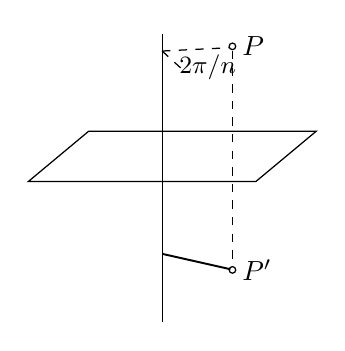
\begin{tikzpicture}[line width=.45pt,scale=.85]
 \draw (-2.0,0)--(1.4,0)--(2.3,.75)--(-1.1,.75)--cycle;
 \draw (0,-2.1)--(0,2.2);
 \filldraw[fill=white] (1.05,2.02) circle (1.4pt) node[right] {$P$};
 \draw[dashed] (0,1.95)--(1.01,2.0);
 \draw[dashed] (0,1.95)--(.34,1.64);
 \node at (.68,1.7) {\small $2\pi/n$};
 \draw[dashed] (1.05,1.95)--(1.05,-1.28);
 \filldraw[fill=white] (1.05,-1.32) circle (1.4pt) node[right] {$P'$};
 \draw[line width=.7pt] (0,-1.08)--(1.02,-1.31);
\end{tikzpicture}
\caption{}
\label{fig:91-32}
\end{figure}

We denote a rotation--reflection transformation by $S_n$. If reflection in the plane normal to the given axis is denoted by $\sigma_h$, then, by definition,
\begin{equation}
S_n=C_n\sigma_h=\sigma_hC_n
\tag{91.4}
\end{equation}
(the outcome evidently does not depend on the order in which $C_n$ and $\sigma_h$ are performed).

The rotation--reflection axis of second order is an important special case. A rotation through $\pi$ followed by reflection in the plane perpendicular to the rotation axis is readily recognized as an \emph{inversion}. Under this transformation a point $P$ of the body goes to another point $P'$ on the continuation of the line joining $P$ to the point $O$ where the axis intersects the plane; moreover, $OP=OP'$.

\SourcePage{432}{435}
A body symmetric under this transformation is said to have a center of symmetry (we shall denote inversion by $I$):
\begin{equation}
I\equiv S_2=C_2\sigma_h.
\tag{91.5}
\end{equation}
It is also plain that $I\sigma_h=C_2$ and $IC_2=\sigma_h$. Thus, a second-order axis, a plane of symmetry normal to it, and a center of symmetry at their intersection are mutually dependent: the presence of any two of these elements necessarily entails the third.

We now note several purely geometrical properties of rotations and reflections that are useful when studying the symmetry of bodies.

The product of two rotations about axes meeting at a point is a rotation about a third axis through that same point. Two reflections in intersecting planes are together equivalent to a rotation. Its axis is clearly the line in which the planes intersect, while its angle, as follows at once from a simple geometrical construction, is twice the angle between the two planes. Let $C(\varphi)$ denote rotation through $\varphi$ about the axis, and let $\sigma_v$ and $\sigma'_v$ denote reflections in two planes containing that axis.\footnote{The subscript $v$ is customarily used for reflection in a plane containing the given axis (a ``vertical'' plane), whereas $h$ denotes reflection in a plane perpendicular to the axis (a ``horizontal'' plane).} The statement just made may then be written
\begin{equation}
\sigma_v\sigma'_v=C(2\varphi),
\tag{91.6}
\end{equation}
where $\varphi$ is the angle between the two planes. The order of the reflections must be observed: $\sigma_v\sigma'_v$ gives a rotation directed from the plane $\sigma'_v$ toward the plane $\sigma_v$, whereas interchanging the factors reverses the sense of rotation. Multiplication of (91.6) on the left by $\sigma_v$ yields
\begin{equation}
\sigma'_v=\sigma_vC(2\varphi);
\tag{91.7}
\end{equation}
in other words, the product of a rotation and reflection in a plane containing the rotation axis is equivalent to reflection in another plane, inclined to the first at an angle equal to half the angle of rotation. In particular, this shows that a second-order symmetry axis and two mutually perpendicular symmetry planes through it are mutually dependent: if two are present, the third must be present as well.

\SourcePage{433}{436}
We shall show that rotations through $\pi$ about two axes that meet at an angle $\varphi$ (the axes $Oa$ and $Ob$ in Fig.~33) have as their product a rotation through $2\varphi$ about the axis perpendicular to both (the line $PP'$ in Fig.~33). The resulting transformation is known in advance to be a rotation. Under the first rotation, about $Oa$, the point $P$ moves to $P'$; under the second, about $Ob$, it returns to its initial position. Consequently, the line $PP'$ remains fixed and is therefore the rotation axis. To find the angle of rotation, observe that the first rotation leaves the axis $Oa$ in place, whereas the second carries it into the position $Oa'$, which makes an angle $2\varphi$ with $Oa$. The same argument shows that reversing the order of the transformations reverses the direction of rotation.

\begin{figure}[ht]
\centering
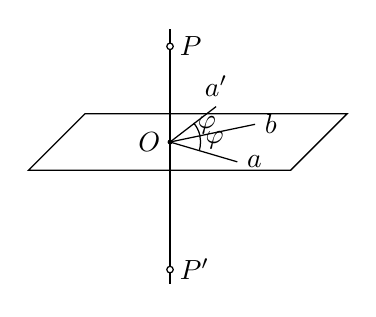
\begin{tikzpicture}[line width=.45pt,scale=.9]
 \draw (-2,0)--(1.7,0)--(2.5,.8)--(-1.2,.8)--cycle;
 \draw (0,-1.6)--(0,2.0);
 \filldraw[fill=white] (0,1.75) circle (1.3pt) node[right] {$P$};
 \filldraw[fill=white] (0,-1.4) circle (1.3pt) node[right] {$P'$};
 \fill (0,.4) circle (1pt) node[left] {$O$};
 \draw (0,.4)--(1.2,.65) node[right] {$b$};
 \draw (0,.4)--(.95,.12) node[right] {$a$};
 \draw (0,.4)--(.65,.9) node[above] {$a'$};
 \draw (.42,.5) arc[start angle=14,end angle=40,radius=.42];
 \draw (.413,.281) arc[start angle=-16,end angle=12,radius=.43];
 \node at (.63,.43) {$\varphi$}; \node at (.52,.63) {$\varphi$};
\end{tikzpicture}
\caption{}
\label{fig:91-33}
\end{figure}

Although the result of two successive transformations generally depends on their order, there are several cases in which the order of operations is immaterial, so that the transformations commute. These cases are:

1) two rotations about the same axis;

2) reflections in two mutually perpendicular planes (their product is equivalent to a rotation through $\pi$ about the line where the planes intersect);

3) rotations through $\pi$ about two mutually perpendicular axes (their product is equivalent to a rotation through the same angle about the third perpendicular axis);

4) a rotation and reflection in a plane perpendicular to its axis;

5) any rotation (or reflection) together with inversion about a point on the rotation axis (or in the reflection plane); this follows from 1) and 4).
